\documentclass[main.tex]{subfiles}

\begin{document}
\chapter{Detailed Design}
\chaplabel{detailedDesign}

The detailed design is a result of a more thorough design process, following the outcomes from the concept design, and will form the basis of the work programs for the project. This detailed design will become the reference point for the construction and development during the build phase of the project, and has been selected as being a time effective and cost effective solution to delivering the project goals. The detailed design has been separated into subsystems which can be developed concurrently, maximising productivity of team members. These subsystems and their designs are detailed below.

\section{Automation}
\seclabel{detailedautomate}

As part of the platform requirements, full autonomy of the vehicle was required. For the quad bike this meant being able to operate each of the subsystems, steering, throttle, gears, and brakes, remotely without human interaction as well as knowing state information about the quad bike including the speed, position and heading. To achieve this the quad bike uses a series of actuators and motors to operate the subsystems in place of human interaction.

\subsection{Platform Modifications}
\seclabel{detailedmodifications}

A visual inspection and individual tests of each of the subsystems revealed a number of hardware and/or software issues. Due to this substantial changes were made to the control, steering, braking, gearing and positioning systems while no changes were made to the throttle and wheel encoder systems.

The original brake system incorporated a limit switch and strain gauge to determine if the brake was actuated. The limit switch limited the brake motion at the extreme limit and the strain gauge dictated the brake intensity and ensured the brake lever was not being over strained. Testing of this system revealed that the brake intensity fluctuated by \textcolor{red}{15 percent NEED TOP CHECK } which would have resulted in inconsistent stopping distances. This was tested by requesting certain braking intensities and measuring the travel distance of the actuator arm and by spinning the wheel. The tests lead to the redesign of the brake measurement for greater accuracy. Improved braking accuracy was achieved through the use of a linear transducer installed on the actuator. This transducer allowed for the travel of the actuator arm to be controlled and for the position to be known to the nearest millimetre. Knowing the position of the actuator arm allows for accurate and uniform brake intensities and thus, braking distances.

As highlighted in the platform requirements, forwards and reverse motion is required for the desired mission profile. A linear actuator in conjunction with two hall effect sensors were used to move the gear selector lever. Hall effect sensors measured the forwards or backwards motion of the actuator and dictated the limits of the motion. Neutral was the position in the middle of the sensors while Drive and Reverse were to the left and right respectively. Selecting Drive or Reverse resulted in the actuator pushing the gear lever to a point until the hall effect sensor reached a certain value and the arduino ordered the actuator to stop.

\subsection{Steering System}
\seclabel{detailedsteering}

\subsection{Automation Software}
\seclabel{detailedautosoftware}

\section{Navigation}
\seclabel{detailednav}
Platform navigation is primarily handled via waypoints. After a region is selected by a user it
is broken down into a series of waypoints which the quad bike will attempt to follow. In the
alternate use case, the user will specify a path directly and the navigation system will operate
directly on these waypoints.
\subsection{Waypoint Generation}
\seclabel{detailedwaypointgen}
The waypoints are generated from a zone of interest to facilitate the autonomous surveying of areas that are suspected to contain mines. This zone must be capable of being user defined to match real world boundaries. The algorithm used to generate these waypoints is a modified linescan algorithm which will be tuned to output scanlines of the same width as the equipment's scan width.

To allow for complex polygonal zones to be entered by the user, the original user-defined polygon boundary is split into a series of convex hulls, simplifying the line scanning algorithm. The split of the user polygon is shown in \Figref{wayPointGeneration}, where the user-defined polygon is outlined in bold blue and the series of generated convex search regions are shaded within. The black path shows the output of the linescan algorithm starting at the origin (marked by the red dot in the south-east corner), and ends at the second red dot at the far end of the path. The linescan algorithm searches for the nearest corner from the nearest convex polygon and begins plotting successive alternating scanlines through the polygon. After a convex polygon has been completely covered, the linescan algorithm connects to the next nearest corner of the next nearest polygon and the process continues. This system allows for multiple user defined regions to be connected and autonomously scanned in a single pass.

\begin{figure}[ht]
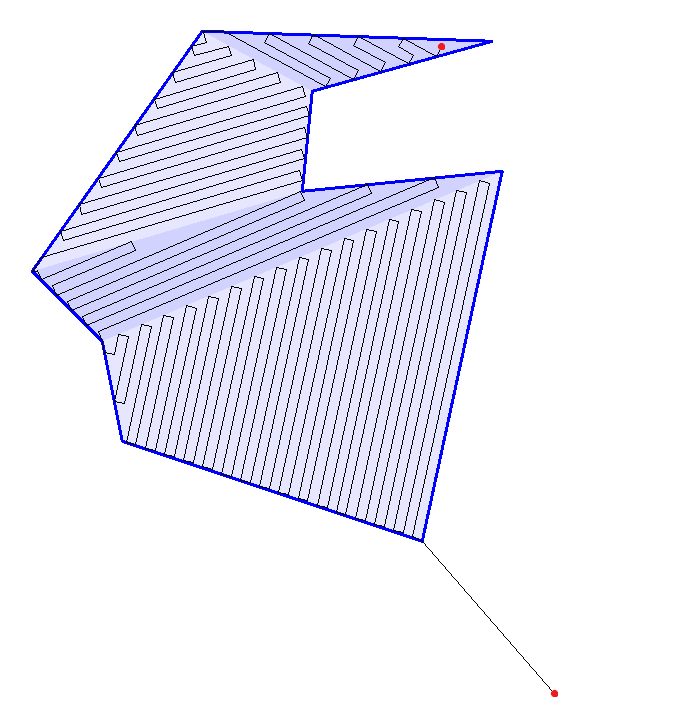
\includegraphics[width=0.5\textwidth]{5-DetailedDesign/lineScanAlgorithm.png}
\centering
\caption{Output of preliminary waypoint generation algorithm} \figlabel{wayPointGeneration}
\end{figure}

\subsection{Low Curvature Path Following}
For low curvature path following (such as a straight line connecting waypoints discussed in \secref{detailedwaypointgen}) Pure Pursuit is used. The tracker works through determining an arc that connects the non steering wheel axle to a goal point on the path (refer back to \Figref{purePursuitGeom}).  The goal point ($g_x, g_y$) acts as an intermediate waypoint and is determined from a look-ahead distance $l_d$. The angle, $\alpha$, can be related to the geometry using the law of sines,
\begin{align*}
\frac{l_d}{\sin(2\alpha)} &= \frac{R}{\sin(^{\pi}/_2-\alpha)},\\
\frac{l_d}{2\sin(\alpha)\cos(\alpha)} &= \frac{R}{\cos(\alpha)},\\
\frac{l_d}{2\sin(\alpha)} &= R.
\end{align*}
Then the steer angle, $\delta$, can be determined from the geometry shown in \Figref{geometricBicycleModel} where
\begin{figure}[ht]
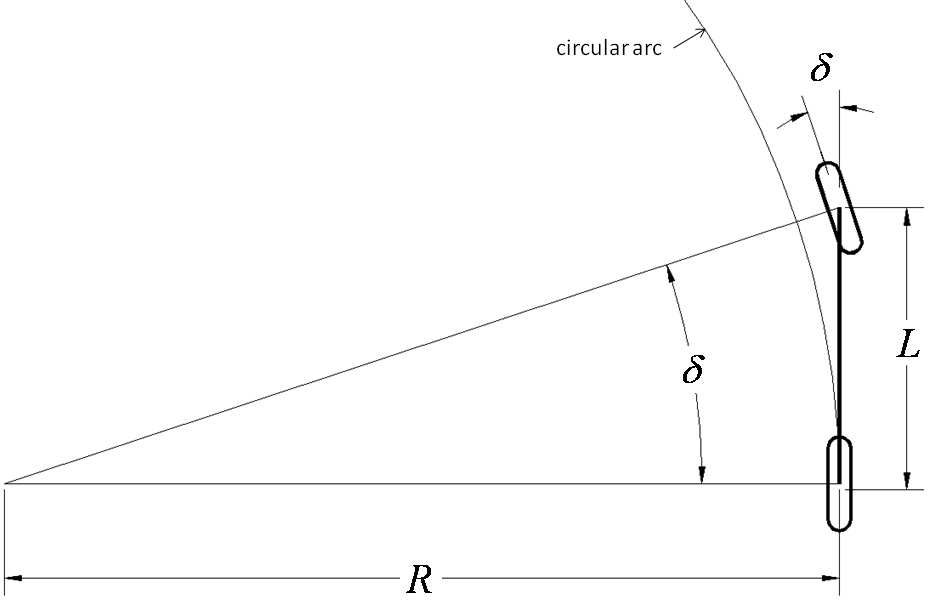
\includegraphics[width=0.7\textwidth]{5-DetailedDesign/Geometric_Bicycle_Model.png}
\centering
\caption{Geometric bicycle model} \figlabel{geometricBicycleModel}
\end{figure} 
\begin{align*}
R &= \frac{l_d}{2\sin(\alpha)},
\shortintertext{and the pure pursuit controller is given as}
\delta &= \tan^{-1}\Bigg(\frac{2L\sin(\alpha)}{l_d}\Bigg)
\end{align*}
where $\alpha$ and thus $\delta$ will be functions of time (calculated in real time in practice).
A separate algorithm is used for turning a specified angle due to real quad bike geometry where a minimum turn radius is introduced.

\subsection{Turning the Platform a Specified Angle}
It is evident from \Figref{wayPointGeneration} that many sudden and sharp turns will be encountered during the navigation process. If the quad bike is not to stray a great distance from the path, the pure pursuit method breaks down due to turn angle limitations on the quad bike.  In these situations one of two methods will be used to turn the angle, an N-point turn or a gradual turn \textcolor{red}{INSERT PICTURE HERE!}. If the turn angle is below a user-set threshold a gradual turn will be conducted else an N-point turn will be used.

\subsection{Positioning System}
The requirements for the positioning system were set primarily by the virtual platform (see \textcolor{red}{SECTION NUMBER!!!}). Two requirements were defined for the design, low positional drift and high accuracy. The drift is the speed at which the cartesian position moves relative to the real quad bike position and accuracy is the distance error of the positioning system from the real quad position. The maximum allowable drift for the system was defined as 0.2 m/s, speeds exceeding this resulted in irregular steering motor fluctuations either side of the desired steering angle. The minimum allowable accuracy was defined as 0.5 m as set in the project specifications \textcolor{red}{NEED TO ADD THIS TO THE PROJECT SPECIFICATIONS}.

To satisfy these characteristics an Extended Kalman Filter (EKF) was employed to fuse the data from two positional sources, a GPS and IMU, and quad bike kinematic equations. It is capable of taking in to account the noise and inaccuracies from multiple measurements to produce an output which is likely more accurate than each of the individual readings. The EKF is defined as follows:
\begin{align*}
\shortintertext{Prediction Equations:}
&\bar{\mu_t} = g(u_t, \mu_{t-1}) + \delta_t\\
&\bar{\Sigma_t} = G_t\Sigma_tG_t^T + R_t\\
\shortintertext{Update Equations:}
&z_t = h(\mu_t) + v_t\\
&K_t = \bar{\Sigma_t}H_t^T(H_t\bar{\Sigma_t}H_t^T + Q_t)^{-1}\\
&\mu_t = \bar{\mu_t} + K_t(z_t-h(\bar{\mu_t}))\\
&\Sigma_t = (I - K_tH_t)\bar{\Sigma_t}
\end{align*}
Where the state vector, $\mu_t$, holds the positional information ($x, y, \theta$) in a 3x1 matrix. The EKF is calculated in two steps, a prediction step and an update step. The prediction step uses kinematic equations to update the position of the quad bike based on physical observations. In the case of the quad bike, readings of the velocity, steering angle and time-step are taken, then geometry is used to calculate where its updated position would be. The update step then uses information obtained through sensors to correct for any error that may be present in the prediction step. This is achieved by modelling positions as a Gaussian distribution and weighting them according to their reliability. Gaussian distributions are shown as covariance matrices, $R_t$ for the prediction step and $Q_t$ for the update step, and the weighting is the Kalman Gain, $K_t$. The predicted covariance matrix, $\Sigma_t$, can then be determined. As we know the starting position and heading of the quad bike through user input, $\Sigma_t$ is initialised as a 3x3 zero matrix.

A visual representation of the kinematic equations used are shown in \figref{quadKinematics}, where:
\begin{align*}
&R = \frac{L}{tan\ \delta}\\
&\phi = \frac{V\Delta t}{R}\\
&y_q = Rsin\phi\\
&x_q = R(1-cos\phi)
\shortintertext{and in the global frame:}
&x_G = y_qsin\theta + x_qcos\theta\\
&y_G = y_qcos\theta + x_qsin\theta\\
&\theta = \theta + \phi
\end{align*}
\begin{figure}[ht]
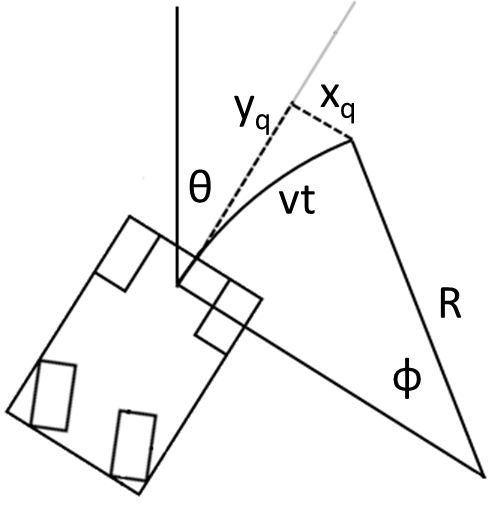
\includegraphics[width=0.5\textwidth]{5-DetailedDesign/quadbikeKinematics.png}
\centering
\caption{quad bike Kinematics} \figlabel{quadKinematics}
\end{figure} 
so the prediction equation for $\bar{\mu_t},\ g(u_t,\ \mu_{t-1})$ becomes:
\[
g(u_t, \mu_{t-1}) =
\begin{bmatrix}
	x_G + y_qsin\theta + x_qcos\theta\\
    y_G + y_qcos\theta + x_qsin\theta\\
    \theta + \phi
\end{bmatrix}
\textrm{, } G = \frac{\partial g_i}{\partial x_j} =
\begin{bmatrix}
    1	&	0	&	y_qcos\theta - x_qsin\theta\\
    0	&	1	&	-y_qsin\theta - x_qcos\theta\\
    0	&	0	&	1
\end{bmatrix}
\]
This needs to be recalculated at each prediction step as well as it's Jacobin, $G$. The process noise for the prediction, $\delta_t$, is represented by a Gaussian distribution with covariance $R$.
\[
R =
\begin{bmatrix}
    \sigma_x^2	&	0	&	0\\
    0	&	\sigma_y^2	&	0\\
    0	&	0	&	\sigma_\theta^2
\end{bmatrix}
=
\begin{bmatrix}
    (0.025 \times V\Delta t)^2	&	0	&	0\\
    0	&	(0.025 \times V\Delta t)^2	&	0\\
    0	&	0	&	(0.97 \times V\Delta t)^2
\end{bmatrix}
\]
Where $\sigma_x, \sigma_y, \textrm{and } \sigma_\theta$ are based on the accuracy of readings given by the velocity and steer angle sensors on the quad bike. Testing (\textcolor{red}{INSERT SECTION}) showed the error in distance, ($\sigma_x, \sigma_y$), to consistently vary within 0.5 m for every 20 m travelled, or 0.025 m/m. Since the heading is calculated based on the distance travelled and the turn angle, the error is also dependent on these factors. The steering motor is accurate to 1 degree of the true value due to initialisation and the error is maximum when at full lock due to the trigonometric function present in the turn angle equation below. The difference in turn angle at full lock when a 1 degree error is present is then:
\begin{align*}
&\Delta\phi = \frac{V\Delta t}{\frac{L}{tan\ 24}} - \frac{V\Delta t}{\frac{L}{tan\ 23}} = \frac{V\Delta t}{2.87} - \frac{V\Delta t}{3.02} = 0.017V\Delta t = 0.97\ \degree/m
\end{align*}
Information from two sensors are observed, positional and angular data from the GPS and angular data from the IMU. In the case of the GPS, the EKF inputs are the observation matrix and its Jacobian:
\[
h(\mu_t) = \mu_t = 
\begin{bmatrix}
    x_{gps}\\
    y_{gps}\\
    \theta_{gps}
\end{bmatrix}
\textrm{, } H = \frac{\partial h_i}{\partial x_j} = 
\begin{bmatrix}
    1	&	0	&	0\\
    0	&	1	&	0\\
    0	&	0	&	1
\end{bmatrix}
\]
And an observation error modeled by a Gaussian distribution with covariance matrix $Q$:
\[
Q = 
\begin{bmatrix}
    \sigma_x^2	&	0	&	0\\
    0	&	\sigma_y^2	&	0\\
    0	&	0	&	\sigma_\theta^2
\end{bmatrix}
=
\begin{bmatrix}
    0.4^2	&	0	&	0\\
    0	&	0.4^2	&	0\\
    0	&	0	&	20^2
\end{bmatrix}
\]
As the GPS drifts when stationary, positional data from this sensor is only used when the platform is at cruising speed, or when travelling in a forwards direction at 5 km/hr. Experimental data showed the GPS to be accurate within 0.4 m at this speed, and therefore the calculated heading accurate within ~20 degrees when measuring between subsequent points. 

The IMU is also used to correct the heading and as only one element of the state vector is being updated the matrix math is set up slightly differently. Experimental data shows the IMU has an error of approximately 2 degrees per 360 degrees travelled. 
\[
h(\mu_t) = \mu_t = 
\begin{bmatrix}
    \theta + \Delta \theta_{imu}
\end{bmatrix}
\textrm{, } H = \frac{\partial h_i}{\partial x_j} = 
\begin{bmatrix}
    0	&	0	&	1
\end{bmatrix}
\]
And an observation error modeled by a Gaussian distribution with covariance matrix $Q$:
\[
Q = 
\begin{bmatrix}
    \sigma_\theta^2
\end{bmatrix}
=
\begin{bmatrix}
    (\frac{2}{360}\Delta \theta_{imu})^2
\end{bmatrix}
\]
With the inputs calculated a new estimate covariance and position estimate is outputted. 
\Figref{kalmanError} shows the x and y components of the distance error from the true value for the Kalman filtered position and the position from kinematic equations. The simulation consisted of a 25 degree right turn, 25 degree left turn, followed by a long straight beginning at the nine second mark. Due to the certain starting position of the quad bike the errors all begin at zero. We can see that when using the kinematic equations alone, the error grows due to the additive nature of the process. A diverging result occurs because the heading calculated through kinematics is not the true heading. When corrected with the IMU and GPS the Kalman position stabilises and the error peaks at approximately 0.4 meters, which is within specifications.
\begin{figure}[ht]
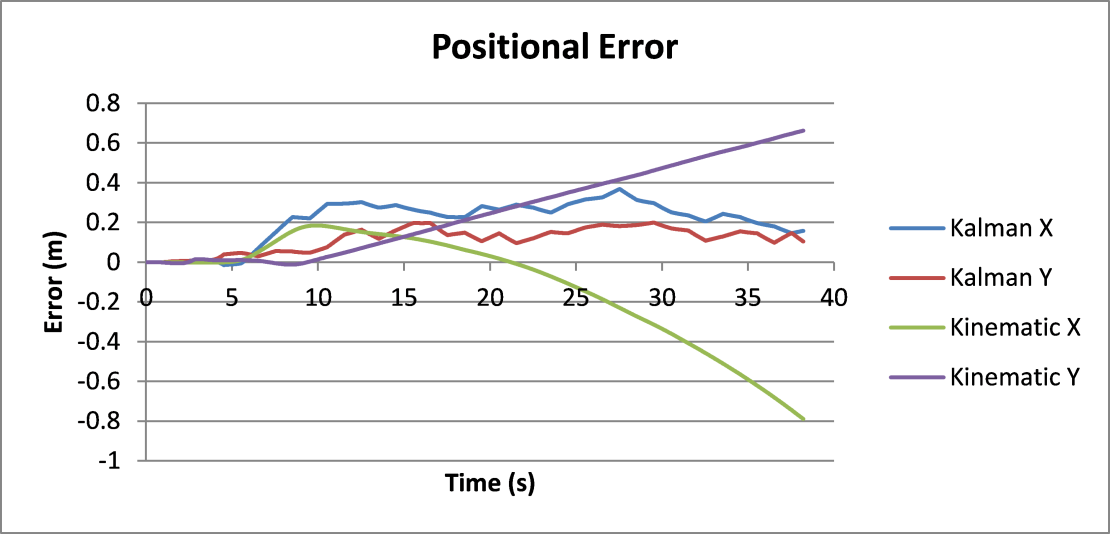
\includegraphics[width=\textwidth]{5-DetailedDesign/KalmanErrorGraph.png}
\centering
\caption{Error of positional estimates from virtual platform simulation} \figlabel{kalmanError}
\end{figure} 

\section{Sensor Mount}
Both the GPR and metal detector are required to be mounted to the platform in a cantilever-like fashion in order to avoid contact with the ground where it would risk detonation of a landmine. Each of the sensor arrays is expected to weigh between 10 kg and 30 kg.
Mounting needs to be done in a configuration that will keep individual array sensors aligned so that corresponding ground information can be collated and analysed correctly. If the assumption of Ackermann steering holds for the quad bike we can use the simplified, 2-wheel model to assess the location of the sensors relative to the quad bike. The simplified model provides the following geometric relationship:
$$
tan(\delta) = \frac{L}{R}
$$
Where $\delta$ is the steering angle, $L$ is the wheelbase and $R$ is the radius of the arc that the centre of the rear axle will follow. This simplification has been used to perform simulations on the steering effectiveness of the vehicle and will also be used to estimate turning capabilities as part of the route planning software.
Initial simulations showed that front mounted sensors with rear-wheel steering is the best option for the application with far superior coverage results compared to front-wheel steering. Further results are shown in \Figref{turnCoverage}
\begin{itemize}
\item Trial 1, represented as the leftmost diagram in \Figref{turnCoverage}, shows the turning example for a case where the turning wheels are 1.5 metres in front of the focal point of the turn, or front wheel steering. The sensor array is 0.5 metres in front of the turning wheels, 2 metres from the focal point of the turn. Evident from the figure is how the coverage area does not form a tight loop and the coverage area does not include the path of the vehicle. This is critical as it will mean the quad bike will be passing over ground not scanned by the sensors.
\item Trial 2, represented by the middle diagram in \Figref{turnCoverage}, shows the results for a case where the turning wheels are 1.5 metres behind the focal point of the turn, or rear wheel steering. The sensor array is placed 0.5 metres in front of the focal axle. This trial shows a much tighter scanning loop than the previous test and the path of the quad bike is entirely within the scanned area. This is ideal.
\item The third trial, represented by the rightmost diagram in \Figref{turnCoverage}, is purely for comparison and shows the coverage area of a vehicle with turning wheels 1.5 metres in front of the focal axle, but with the sensing array only 0.5 metres in front of the focal axle. This would place the sensing array between the two axles of the vehicle. Under this arrangement an identical scanning path is achieved using a front-wheel steering setup. This is not useful for the application as the sensors must be in front of the vehicle to detect landmines.
\end{itemize}
% Split, subfig
\begin{figure}[ht]
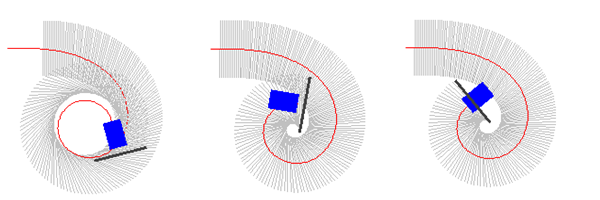
\includegraphics[width=0.8\textwidth]{5-DetailedDesign/Detector_Coverage.png}
\centering
\caption{Mine detector coverage simulations} \figlabel{turnCoverage}
\end{figure}
This result is expected. Referring to \Figref{geometricBicycleModel}, the turning radius of the rear wheel is $R$ and the turning radius of the front wheel is the hypotenuse of the triangle formed – of length $\sqrt{R^2 + L^2}$, which is greater than $R$. If the sensing array was some distance $q$ in front of the front wheels, its turning radius would be $\sqrt{R^2 + [L+q]^2}$, greater yet again. However, if the sensing array was an equal distance $q$ behind the rear wheels (or front wheels if this was a rear-steering arrangement) then the turning radius of the sensors would be $\sqrt{R^2 + q^2}$. From this it can be seen that to minimise the effective turning radius then $q$ should be minimised.

The sensor arrays will be mounted at the 'rear' of the quad bike which will be primarily driven in reverse to achieve the desired scan coverage. The mounting bracket for the arrays will be constructed on-the-fly with the assistance of the workshop and its technicians. The bracket should be constructed from PVC and meet the following specifications:
\begin{itemize}
\item Metal detector clear of metal in a 500 mm radius and 2000 mm vertically.
\item GPR clear of obstructions in a 100 mm radius and 50 mm vertically.
\end{itemize}

\subsubsection{Final sensor mount design}
For the final design for the sensor mount to adhere to all the sensory requirements, design tests were required to be conducted. These tests were necessary to test for variations in ground clearances and vibrational interference from the Quad bike during operation. Testing for these were carried out using the Finite Element Analysis (FEA) method and engine run tests on the quad bike. FEA was used to test vibrational harmonics and load carrying ability of the frame when subject to operational conditions while engine run tests were used to test the vibrational frequency of the operating quad bike. 

\subsubsection{FEA}
The sensor frame design was constructed in FEA. The FEA methods discretises a geometry into a finite number of elements connected together via nodes. Boundary conditions, loads and constraints as well as material properties are subject to the design and depending on the analysis type, a result can be interpreted that can be used to alter and fine tune the design.  To properly and accurately model the frame, 3D elements were chosen to represent the geometry and a basic load test was conducted. This load test was conducted to ensure that the deflection of the mount when subject to the weight of the sensor systems would not interfere with the sensor requirements, and to check if the design was strong enough to support the weight. 

talk about load test, talk about hand calc verification

then talk about vibrational test using harmonic analysis. discuss results. discuss vibration expected- vibration tests during engine tests, theoretical vibration tests for driving
any alterations made to the design

Picture of our final design in CAD and FEA and irl



    

\section{Signal Processing}
\seclabel{signaldetailed}


As per the concept design, the signal processing subsystem will be based on a weighted evaluation of the sensor data to achieve the goal of reporting a confidence level for the existence of mines.
The weighted evaluation will be the combination of three detection algorithms utilising two sensors. Each independent algorithm will be capable of reporting some confidence in the existence of a mine object, with the combination expected to improve the detection rate and reduce the number of false positives.

The development process is expected to be highly experimental and involve a significant degree of manual tuning or collection of datasets to produce quality results. The time required to complete these tasks is unknown due to their experimental nature, as so an agile development strategy is proposed. Under the agile software development strategy, software is developed incrementally without explicit milestones being set prior to commencement. After each incremental stage of the software production is completed, a re-evaluation process is used to develop the next project milestone and the expectations for project completion are adjusted and documented. This strategy is expected to ensure the software deliverable has some baseline capabilities at project end, in the event that the full software goals are not met. This is in contrast to other development strategies which are highly structured and may result in completion of individual modules, but delivery of a non-functional combined product in the event that project timeframes are not met as expected.

Using the agile development strategy, project development is planned to continue as follows, with each element being completed before progress commences on the next item:
\begin{itemize}
\item Initialisation of sensor devices and collection of information into suitable data structures. The proposed data collection arrangement is shown in \Figref{datamanagement}.
\item Processing of data with a single algorithm (of the three selected) using arbitrary success criteria to indicate presence of a mine.
\item Training of the completed single algorithm system with actual sample data, either manually or using a computer learning method, depending on a progress evaluation at commencement of this task.
\item Commencement of development and software training for additional algorithms
\item Development and training of a machine learning algorithm to determine mine probability from the outputs of the three independent algorithms.
\end{itemize}

The tasks as they appear above may be modified during project development or postponed indefinitely, as is inline with the agile development strategy. As such the detailed design extends to the second item in the previous list, corresponding to the first stage at which the software will meet the deliverable requirements. Future design outlines will be completed at evaluation stages as the project progresses.

\begin{figure}[ht]
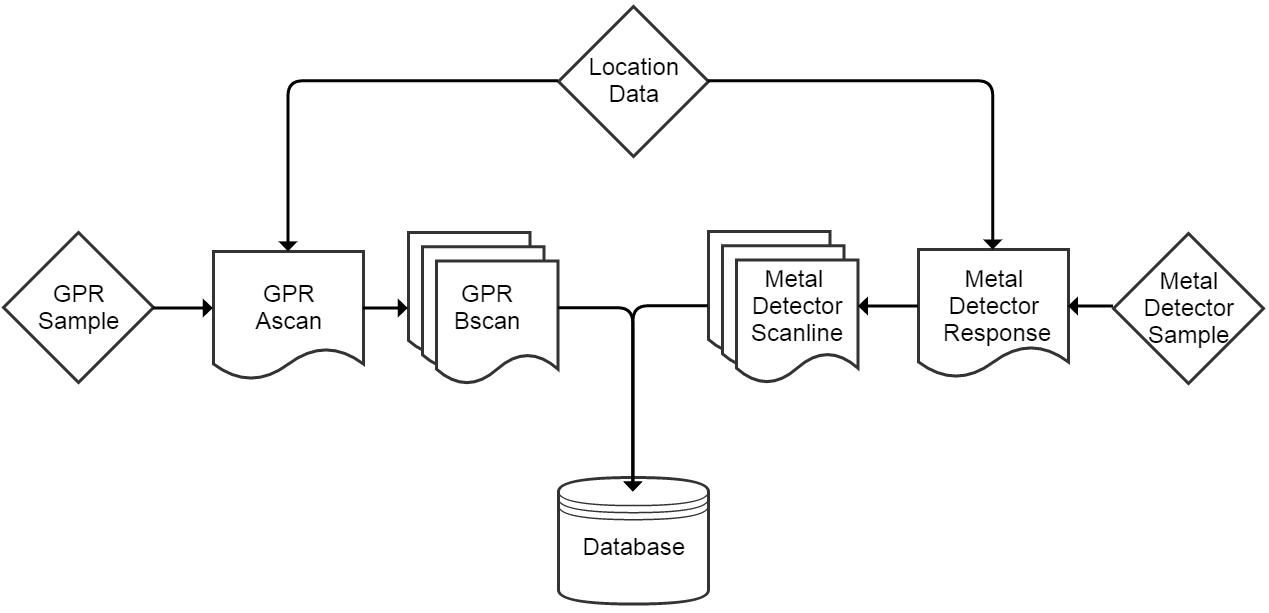
\includegraphics[width=\textwidth]{5-DetailedDesign/data-management.png}
\centering
\caption{Data collection strategy for the signal processing system}
\figlabel{datamanagement}
\end{figure}

The program flow design for the completion of the first detection algorithm is shown in \Figref{agile}. The first algorithm to be attempted is the identification of feature parabolas using the randomised Hough transform over the GPR B-scan, as this method produces a visual output which can easily be tested for correctness by an operator by visual comparison. It will also involve the development of the background signal isolation process, which will also be able to be visually inspected for correctness and will be required for the preprocessing steps of the other detection algorithms.
Once the Feature Parabolas have been isolated from the received signal, criteria will be determined by a human operator which will be used to provide classification between mines and non-mine objects.

\begin{figure}[ht]
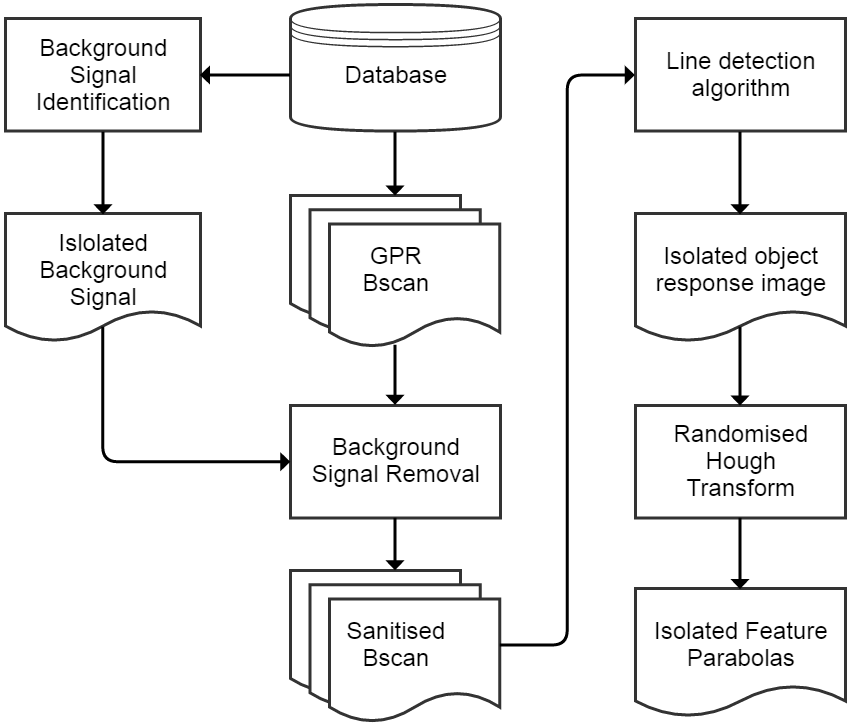
\includegraphics[width=0.8\textwidth]{5-DetailedDesign/agile-strategy.png}
\centering
\caption{Software program flow for initial development stage}
\figlabel{agile}
\end{figure}

\section{Electronics Hardware}
The electronics hardware to be used for the project will fit in the categories as described in the Conceptual Design. The custom electronics work pre-existing on the quad bike supplied by the DSTG meets the requirements for the COTS bespoke electronics, providing digital interfaces to the actuators and sensors attached to the platform. The need for replacement or improvement of any of these electronics will be determined after testing has been completed on the supplied vehicle and their performance has been evaluated.

As the electronics system does not have particularly strict requirements for part selection, and due to the COTS equipment being mostly interchangeable with little effect on appropriateness for the project, the electronics hardware has been chosen on a basis of what is most readily available to the project and most familiar to the project members. This choice reduces time spent in the design stage and allows for a rapid development process to commence as early as possible.

The central processing hardware will be provided by a Windows based desktop computer supplied by the University of Adelaide. A Windows device has been chosen to be able to make use of the provided drivers for the GPR system which are only compatible with 32-bit Windows machines. The selected device has WiFi communications capabilities and dedicated serial communications ports, allowing easy communications to a microcontroller device providing low level I/O.

The microcontroller selected is an Arduino Mega 2560 board, chosen for its cost, availability and fast development time. This board has considerable I/O capabilities that exceed the requirements for the project, but allow for future expansion of sensors and ensures that I/O limitations will not be a concern. The microcontroller will be connected to the desktop computer via the serial port as mentioned above.

\end{document}
































